

\documentclass[../thesis.tex]{subfiles}

% Documents that contain labels for references in this chapter
\myexternaldocument{Sections/Introduction}

\begin{document}

\section{RQa, how do we measure the energy consumption}
Measuring the power consumption of a program is not as easy as it seems. Measuring the power consumption of the processor as a whole can be done with tools provide by the manufacturer. Measuring the power consumption of one single program is harder. Programs often spawn multiple processes. Besides, measuring the power consumption of the processor as a whole can be done, but a processor is often working on multiple subprocesses of different programs by quickly switching between them. On top of that, modern processors have multiple cores that also alternate between subprocesses. Keeping track on which process is using the processor is proven to be quite challenging. To find a program suitable for this case I did a literature search. Rieger et al. have done a survey on approaches for assessing software energy consumption. While their literature was not performed in a systematic way, they nevertheless are confident that they gained a representative overview of the field and their conclusion was significant:

\begin{quote}
    \emph{"The sobering result of this survey was that there are hardly any actual ready-to-use development tools; those that we found are all platform-specific."} \parencite[p. 24]{rieger2017}
\end{quote}

To still find a way to measure the energy consumption of Cheetah I did a small literature search on how other authors measure energy or power consumption. Some approaches described are from the survey of Rieger et al., some are from a thesis from a master student \parencite{strempel2021}. Other approaches are found seperately. \paragraph{}

Liu et al. \parencite*{liu2022} proposed Leia, a lightweight cryptographic NN inference system at the edge. They implemented their solution on a Raspberry Pi and tested it with a COOWOO power meter. Tian et al. \parencite*{tian2021} proposed an edge computing-assisted framework to boost efficiency of DNN inference tasks on IoT devices that also protect the privacy of IoT data. They implemented it on a Raspberry Pi (client) and MacBook Pro (server) and measured the power consumption of the client with a Powerjive USB multimeter. Wang et al. \parencite*{wang2019} proposed an DNN accelerator against a model inversion attack, implemented their architecture on micro-architectural units and used a SMIC standard-cell library to obtain the energy consumption of the hardware logical units. Other solutions like the Linux tool PowerTOP\footnote{\url{https://github.com/fenrus75/powertop} (accessed on 22-12-22)} can only measure the power on battery powered devices. These approaches use hardware specific solutions, that I unfortunately do not have access to.

Seo et al. \parencite*{seo2008} created a framework for Java-based software systems. Couto et al. \parencite*{couto2015} provide Green Droid: a tool that measures energy consumption of Android programs at run-time. Liu provided a framework, jRAPL\footnote{\url{https://github.com/kliu20/jRAPL} (accessed on 22-12-22)} based on RAPL that can measure energy consumption on Java programs. The Spirals research group provided a framework, PyRAPL\footnote{\url{https://github.com/powerapi-ng/pyRAPL} (accessed on 22-12-22)}, that can measure the energy consumption of Python programs. These approaches are language specific. Cheetah is mostly written in C++ and these approaches do therefore not satisfy as a solution to measure energy consumption.

Chen et al. have proposed Eyeriss \parencite{chen2016, chen20162}, a program that can estimate the power usage based on the structure of the NN and its data flow. Yang et al. \parencite*{yang2016} improved this concept and provided a website\footnote{\url{https://energyestimation.mit.edu/} (accessed on 22-12-22)} but this tool estimates power consumption based on the architecture of a NN. Because this solution is based on the structure of the NN and not on code or programs will this solution not be usefull as a solution.

Santos et al. \parencite*{santos2017} suggest a method to measure the energy consumption using Low Level Virtual Machine and Clang tooling. They tested their methods on two open source systems but their implementation is not open source. One other user created a program\footnote{\url{https://gitlab.com/MarcoCouto/c-lem} (accessed on 22-12-22)} that can measure energy of C programs but did not provide installation instructions. Lastly I found PCM-Monitor\footnote{\url{https://github.com/intel/pcm} (accessed on 22-12-22)} for Intel devices but unfortunately I could not get it working on my own setup. 

\subsection{Scaphandre}
\begin{figure}
    \centering
    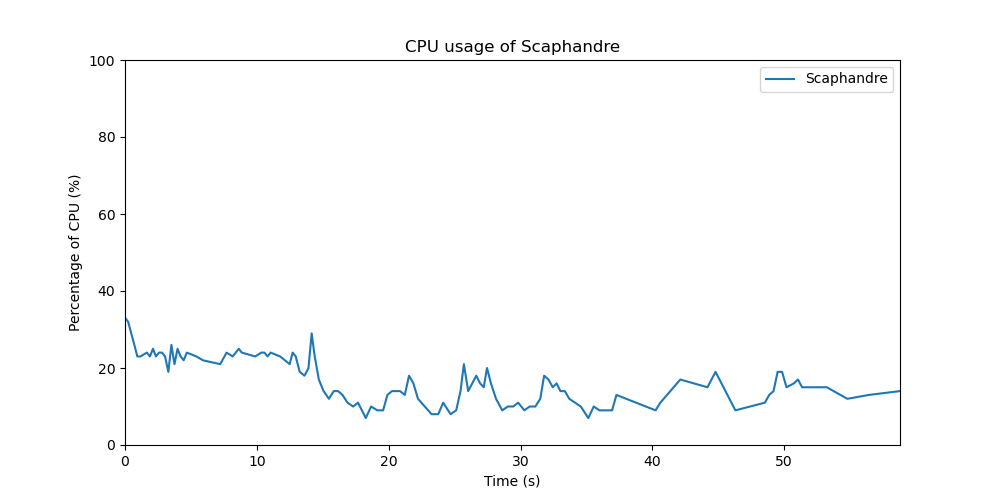
\includegraphics[width=\linewidth]{Thesis/Images/overhead_scaphandre.png}
    \caption{The CPU usage of the process Scaphandre on a test run (while also running the Cheetah process for client an server.}
    \label{fig:overhead_scaphandre}
\end{figure}
I then found Scaphandre, an metrology agent to measure power consumption. I will use Scaphandre for several reasons. Firstly, it is open source\footnote{\url{https://github.com/hubblo-org/scaphandre} (accessed on 22-12-22). For this project I will use commit of the main branch 50fea42 (\url{https://github.com/hubblo-org/scaphandre/commit/50fea42})}, accessible and has a lot of documentation plus an installation guide\footnote{\url{https://hubblo-org.github.io/scaphandre-documentation/} (accessed 23-12-22)}. Although it is an early stage project and is still being maintained it does provide a stable version to work with. Second, Scaphandre measures the energy consumption of specific programs and aims to be as light and clean as possible. Their goal is to reach an overhead as close as possible to 0. Early measurements show that the power consumption is indeed low (Figure \ref{fig:overhead_scaphandre}). Third, Scaphandre outputs the data in convenient forms. It provides support for open source output programs like Prometheus\footnote{\url{https://prometheus.io/} (accessed 23-12-22)}, Riemann\footnote{\url{https://github.com/riemann/riemann} (accessed 23-12-22)} and Warp10\footnote{\url{https://github.com/senx/warp10-platform} (accessed 23-12-22)}. The power consumption metrics can also be stored in a JSON file and basic metrics can be shown to the terminal. \paragraph{}

% begin writing about scaphandre

The process time (total time a process uses the CPU) in Linux is measured in Jiffies. Jiffies are measured in Hz and on most devices 1 second equals 100 Jiffies. Each program keeps track on how many Jiffies it has used. Scaphandre collects this data.

\color{red} Add graph Jiffies => add graph power consumption => add graph total power consumption proces\color{black}

It then combines this data with data collected about the total power used for the machine (for example with Intel's RAPL sensors). The power usage of a program is then calculated as the total power usage multiplied with the ratio between the total Jiffies and the Jiffies used for our program: $ P_{prog} = P_{machine} * \frac{Jiffies_{prog}}{Jiffies_{total}}$. For example: if the total amount of jiffies in a given time period (user and system) is 450 jiffies (sampled per second), and the CPU time of this program (user, system and children) is 50 jiffies, the power usage is then calculated as $P_{prog} = P_{machine} * \frac{50}{450}$. So the power usage of this program will then be $11.11\%$ of the total power usage of the device in that given time period.

% - documentation https://hubblo-org.github.io/scaphandre-documentation/index.html

% Using last commit on the main branch 50fea42 | https://github.com/hubblo-org/scaphandre/commits/main



% \color{red}\textbf{Also notes}\color{black}
% [Solution?] Scaphandre
% https://github.com/hubblo-org/scaphandre/
% measure power consumptoin of tech services and get data in a convenient form
% examples can be found here: https://metrics.hubblo.org/d/GOHnbBO7z/scaphandre?orgId=1&refresh=15m

% [Solution?] pcm-monitor utility, dont know how to get it working

% =========================================================================================================
% [Hardware]
% https://ieeexplore.ieee.org/stamp/stamp.jsp?tp=&arnumber=9663203
% Leia: A Lightweight Cryptographic Neural Network Inference System at the Edge
%  10.1109/TIFS.2021.3138611

% We implement Leia and deploy it on Raspberry Pi
% Usw COOWOO popwer meter COOWOO USB Digital Power Meter Tester. [Online]. Available:
% http://www.coowootech.com/tools.html [[HARDWARE]]

% ------------

% [Hardware]
% https://ieeexplore.ieee.org/stamp/stamp.jsp?tp=&arnumber=9120239
% The voltage and current are measured using a
% Powerjive USB multimeter and the power is calculated by the
% multiplication of voltage and current

% ------------

% [Java] 
% Chiyoung Seo, Sam Malek, and Nenad Medvidovic. “Component-level energy
% consumption estimation for distributed java-based software systems”. In: Lecture Notes in Computer Science (including subseries Lecture Notes in Artificial Intelligence and Lecture Notes in Bioinformatics) 5282 LNCS (2008). ISSN:
% 16113349. DOI: 10.1007/978-3-540-87891-9\_7.

% ------------

% ////////// GOOGLE //////////////////
% [No open source implementation found]
% https://ceur-ws.org/Vol-1938/paper-san.pdf
% introduce crapl a c rapl tool, no open soure implementation found

% [Theoretical calculation based on data movement, not actual overhead of program]
% https://arxiv.org/pdf/1611.05128.pdf
% With the idea of exploiting data reuse in a multi-level memory hierarchy, Chen et al. [21] have presented a framework that can estimate the energy consumption of a CNN for inference
% [21] Y. Chen, J. Emer, and V. Sze, “Eyeriss: A Spatial Architecture for Energy-Efficient Dataflow for Convolutional Neural Networks,” in ISCA, 2016.
% [22] Y. Chen, T. Krishna, J. Emer, and V. Sze, “Eyeriss: An Energy-Efficient Reconfigurable Accelerator for Deep Convolutional Neural Networks,” in ISSCC, 2016.

% [Hardware]
% https://dl.acm.org/doi/pdf/10.1145/3310273.3323070

% ////////// Survey //////////////////
% https://dl.acm.org/doi/pdf/10.1145/3141842.3141846
% Survey of Approaches for Assessing Software Energy Consumption

% [Hardware] Silicon Labs [19] provide an Eclipse-based IDE and development boards for ARM Cortex microcontrollers that allow measuring and profiling the energy consumption of embedded software at runtime. Energy consumption measurements for each method call are provided in a table. This system is commercially available and uses a low-cost development
% board with fast current and voltage sensors. The processor’s program counter is read periodically and its value is sent to the host computer along with voltage and current
% measurements. The program running on the microcontroller is statically linked, uploaded by the host computer and resides at a previously known and constant address in memory. Hence, the address of the program counter is sufficient to infer the currently executed method.

% [Android] Green Droid [3] instruments Android programs and uses PowerTutor [24] to measure their energy consumption at runtime. A trace of the instrumented program and the measured energy consumption are then used to create visualizations in the form of diagrams. These visualizations can help programmers to identify parts of their applications with problematic energy behaviour. To measure energy consumption, PowerTutor relies on a component-based model of the device’s energy usage that can be automatically generated by running a calibration program on the device under test 

% [Java] ELens [10] annotates Java source code for Android with energy consumption estimates. An IDE visualizes this by coloring code according to its estimated energy consumption. The estimates are derived from an instruction-level energy consumption model with path dependencies that has been created by the authors for some specific device.  Evaluating this approach with actual energy measurements gives an accuracy error of about 10\% for methods that run longer than 10ms. Methods with a runtime of less than 10ms could not be measured by the setup used by the authors ( https://ieeexplore.ieee.org/stamp/stamp.jsp?tp=&arnumber=6606555 eLens for android applications)

% Hardly any implementations found, a lot of approaches. While literature and too lsearch was not performed in a very systematic way
% However, we can report that there is a peak of literature on the energy consumption in Android systems. 

% //////////// Thesis //////////////////
% https://ul.qucosa.de/api/qucosa%3A77194/attachment/ATT-0/
% The software scope is chosen because it does not require extra hardware,
% e. g. an ampere meter, to take measurements

% Measurements can be taken in Joule or Watt. These units can be used interchangeably
% when the time frame is known. It is generally advised to use Joule for small and timelimited measurements like the energy usage of a function. Watt is better suited for
% longer or indefinitely running program

% Power = energy/time

% Instant power measurements require extra hardware
% Time measurement is based on the drainage of the energy stored in a battery. Laptops are ideally suited for this technique because they are equiped with integrated batery.
% Creating model can remove biggest disadvantage: namely the dependency on physical instrumentation. Isolate energy consumption of single application.  

% [Java and linux only]
% https://github.com/kliu20/jRAPL
% Can only measure energy consumption on linux

% [Python and not program specific]
% https://github.com/powerapi-ng/pyRAPL
% calculates global energy consumption of all the processes running on the machine. 

% [Linux only]
% https://github.com/kentcz/rapl-tools
% ./AppPowerMeter sleep 5
% will measure the total energy and average power of the CPU while it runs "sleep 5". The CPU power is sampled every 100ms then written to rapl.csv.

% [not program specific]
% https://github.com/sosy-lab/cpu-energy-meter

% [Only battery devices]
% PowerTOP

% [Possible but no documentation]
% https://gitlab.com/MarcoCouto/c-lem\section{Design of experiments}
\section{Experimental setup}
The experiments done are twofold. First, the SNNI's are started on one device. We can then see how the power and energy usage are distributed over time. The tests on one device will show the bare power and energy consumption without limitations on communication protocols. Both devices communicate over the loopback network on 127.0.0.1 and port 12345. Second, to test the effect of bandwidth on SNNI's I will make a different setup with two devices. Because of the limitations of this project and practical reasons, I will only focus on local experiments. This means the experiments are done over LAN, and not WAN. With this setup I will limit the bandwidth to certain predetermined bandwidths to simulate a WAN. I will elaborate the chosen bandwidths later. I chose to leave the ping out of these experiments, also because of practical reasons. The specifications of the devices that are used for the experiments can be found in table \ref{table:specs}.

\begin{table}[]
    \begin{adjustbox}{width=\columnwidth,center}
        \begin{tabular}{lll}
\hline
					    & Server (/client)                                           & Client                                               \\ \hline
CPU				   & AMD Ryzen 3 3100 (4-core processor)    & Intel Core i3-5005U CPU (4-core processor) @ 2.00GHz \\ \hline
GPU                & AMD Radeon HD 7950                             & Intel HD Graphics 5500 (integrated)                  \\ \hline
RAM               & 2x8GB DDR4 3200MHz C16                    & 2x4GB DDR3 1600MHz                                   \\ \hline
Motherboard & Gigabyte B550 Aorus Pro AC                   & Dell FT9HH                                           \\ \hline
OS                   & Ubuntu 22.04.1 LTS (64-bit)                      & Ubuntu 18.04.6 LTS (64-bit)                          \\ \hline
Network         &                                                                       &  Intel Dual Band Wireless-AC 7265                                   \\ \hline
\end{tabular}
    \end{adjustbox}
    \caption{Specifications of the devices that run server (and in case of the single device experiments also client) and client side}
    \label{table:specs}
\end{table}

For this project I forked the project of Cheetah on GitHub. The commit that has been used is 09fe195\footnote{https://github.com/Alibaba-Gemini-Lab/OpenCheetah/commit/09fe195,  (accessed 24-01-23)}. I made some minor changes to the scripts that start the SNNI process that I will elaborate later, but apart from that no changes have been made to the original project. For Scaphandre I use commit 50fea42\footnote{https://github.com/hubblo-org/scaphandre/commit/50fea42, (accessed 24-01-23)}. There have been no changes made to Scaphandre. For Scaphandre I used the JSON exporter. The reason is twofold. First, it does not rely on secondary programs to display the results, and some of the exporters of Scaphandre do (e.g. the Riemann or Promotheus exporter). Second, it outputs the results in convenient form. The STDOUT exporter for example only outputs the top consumers and only displays the name and the power consumption in Watts, while the JSON exporter also gives extra data like the process id and a timestamp. Collecting the process id is important in the two device scenario, because the client- and server side programs are both called "cheetah" or "sci\_he", so separating this data can be quite challenging without.     

\section{Scripts}
To automate the process of running the tests, I have written some scripts in Bash. The reason for this is that bash provides support for all the terminal commands, like creating, removing and moving files/folders, and with a bash script another script can be launched. The latter is important, because the Cheetah framerwork provides scripts to change the parameters of the SNNI.
%  The scripts from single device differ a bit from the scripts written for the experiments for two devices. This has to do with seperating the client measurements and the server measurements in the case of single device.

\subsection{Both devices}
Scaphandre requires the Linux module \verb|intel_rapl_common|. This module can be loaded with \verb|modprobe intel_rapl_common|. This command requires super user rights, so the script has to be run in sudo mode. I then start Scaphandre. For this I need to specify which exporter I want, which is JSON, as described earlier. After this I need to choose the step duration on which Scaphandre collects and outputs the data. This is possible with the \verb|-n| flag and the \verb|-s| flag. The \verb|-n| flag is the step duration in nano seconds, while the \verb|-s| flag is the step duration in seconds. I chose to set the \verb|-n| flag with 1 which causes Scaphandre to output the data as quickly as possible\footnote{For this to work the step duration in seconds needs to be set to 0.}. A consequence of this is that the time between the measurements is not constant, but we can easily solve this later. Lastly we need to specify the name of the output file, which is different each run. By not setting the \verb|-t| flag the script will run till it is terminated. The commands are then:\\

\noindent\verb|modprobe intel_rapl_common|\\
\verb|./Scaphandre -n 1 -s 0 -f [output_name]|\\

\begin{figure}
    \centering
    \subfile{../Graphs/script}   
    \caption{High-level overview of the scripts used for getting measurements}
    \label{fig:scripts}
\end{figure}

Once Scaphandre has been started, we can launch the (slightly altered) scripts from the Cheetah project to start Cheetah and $SCI_{HE}$, called \textit{run-client.sh} and \textit{run-server.sh}. Both programs, client and server, do have the same name, 'Cheetah' or '$SCI_HE$' (dependent of the SNNI), in the output file of Scaphandre. This is a problem in case of the single device tests, since we need to separate the measurements. This wont be the situation in the case of two different devices, since these experiments output 2 separate files, one for the client and one for the server. This can be solved by altering the \textit{run-client.sh} and \textit{run-server.sh} files.

Now the \textit{run-client.sh} and \textit{run-server.sh} both launch the executable in the folder \verb|build/bin|. This executable is the SNNI protocol, and we are interested in the power consumption of this program. Somehow I need to pass the PID of this program, launched from the \textit{run-client.sh} and \textit{run-server.sh}, back to the main script. It is quite trivial on how to pass parameters to children, i.e. with positional parameters\footnote{https://www.gnu.org/software/bash/manual/html_node/Positional-Parameters.html, (accessed on 22-12-22)}, but passing parameters back to the main script is harder. I solved this by adapting the \textit{run-client.sh} and \textit{run-server.sh} by adding \verb|& PID=$!| after the line that executes the SNNI. I then write this PID to a file that is read by the main script. Then the PID can be used to match the measurements of Scaphandre and further process the data (fig \ref{fig:scripts}). This only has to be done in the case of one device. In the case of two devices, we can just seperate the server and client process by naming the output accordingly, e.g. run\_x\_client or run\_x\_server. 

\subsection{Data processing}
The measurements from Scaphandre are in the following format:

\begin{lstlisting}
[
    {
        "host": {
            "consumption": 26271658.0,
            "timestamp": 1673018149.4180377
        },
        "consumers": [
            {
                "exe": "resnet50-SCI_HE",
                "pid": 28350,
                "consumption": 13206809.0,
                "timestamp": 1673018149.9443746
            },
            {
                "exe": "scaphandre",
                "pid": 28333,
                "consumption": 12473097.0,
                "timestamp": 1673018149.9443104
            },

            ...

            {
                "exe": "systemd",
                "pid": 1,
                "consumption": 0.0,
                "timestamp": 1673018149.9416852
            }
        ]
        "sockets" : []
    },
    {
        ...
    },
    ...
]
\end{lstlisting}

To graph the results we first need to filter the SNNI measurements. This can be done by searching for the name (in this example \verb|resnet50-SCI_HE|) and filtering these reseults in the case of two devices, or searching for the PID's of the server and client process and filtering these results in the case of one device. As seen in the example above, the timestamp is in Unix time\footnote{Seconds from the first of Januari 1970 (UTC) \url{}} Now as said before, the data points are not equidistant. We can solve this by interpolating the results. For this I use the Numpy module \verb|numpy.interp|\footnote{\url{https://numpy.org/doc/stable/reference/generated/numpy.interp.html} (accessed on 26-01-23)}. 



\subsection{Parsing the results}

\textbf{Hello world!}
I will use the commit  for this research.

Bandwith between machines in the CryptFlow2 environment is 377MBps and 40MBps in the lan and wan respectively. 
\end{document}
